
% Figure 1: NISE Five-Layer System Architecture
% Paste this into your LaTeX document

\begin{figure}[!t]
\centering
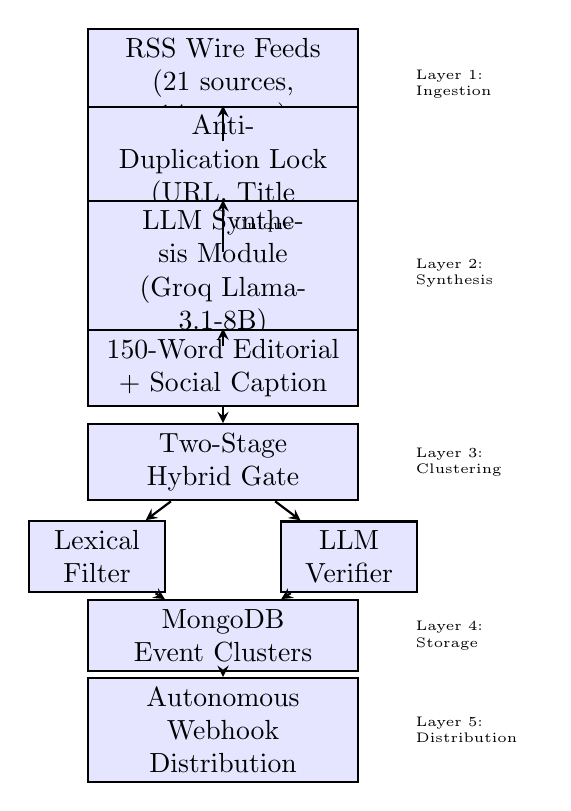
\begin{tikzpicture}[
    node distance=1.2cm,
    box/.style={rectangle, draw, thick, text width=3.2cm, align=center, minimum height=0.8cm, fill=blue!10},
    arrow/.style={->, thick, >=stealth}
]

% Layer 1: Ingestion
\node[box] (rss) {RSS Wire Feeds\\(21 sources, 14 sectors)};
\node[box, below of=rss] (dedup) {Anti-Duplication Lock\\(URL, Title Hash, Title)};

% Layer 2: Synthesis
\node[box, below of=dedup] (llm) {LLM Synthesis Module\\(Groq Llama-3.1-8B)};
\node[box, below of=llm] (summary) {150-Word Editorial\\+ Social Caption};

% Layer 3: Clustering
\node[box, below of=summary] (gate) {Two-Stage Hybrid Gate};
\node[box, below of=gate, xshift=-1.6cm, text width=1.5cm] (lex) {Lexical\\Filter};
\node[box, below of=gate, xshift=1.6cm, text width=1.5cm] (llmv) {LLM\\Verifier};

% Layer 4: Storage
\node[box, below of=gate, yshift=-1cm] (mongo) {MongoDB Event Clusters};

% Layer 5: Distribution
\node[box, below of=mongo] (webhook) {Autonomous Webhook\\Distribution};

% Arrows
\draw[arrow] (rss) -- (dedup);
\draw[arrow] (dedup) -- node[right, font=\tiny] {Unique} (llm);
\draw[arrow] (llm) -- (summary);
\draw[arrow] (summary) -- (gate);
\draw[arrow] (gate) -- (lex);
\draw[arrow] (gate) -- (llmv);
\draw[arrow] (lex) -- (mongo);
\draw[arrow] (llmv) -- (mongo);
\draw[arrow] (mongo) -- (webhook);

% Side annotations
\node[right of=rss, xshift=2cm, font=\tiny, text width=1.5cm] {Layer 1:\\Ingestion};
\node[right of=llm, xshift=2cm, font=\tiny, text width=1.5cm] {Layer 2:\\Synthesis};
\node[right of=gate, xshift=2cm, font=\tiny, text width=1.5cm] {Layer 3:\\Clustering};
\node[right of=mongo, xshift=2cm, font=\tiny, text width=1.5cm] {Layer 4:\\Storage};
\node[right of=webhook, xshift=2cm, font=\tiny, text width=1.5cm] {Layer 5:\\Distribution};

\end{tikzpicture}
\caption{NISE five-layer pipeline architecture. Layer 3 hybrid gate reduces LLM calls by 82.2\% via lexical pre-filtering.}
\label{fig:architecture}
\end{figure}
